\chapter{Hyperparameter Tuning}
\label{chap:hyperparameter_tuning}
\todo{Crossover rate or crossover prob?}
The performance of a Genetic Algorithm is significantly influenced by its control parameters. Performant settings on a particular fitness landscape might not be appropriate an different one (\cite{kacprzyk_parameter_2007}).

According to the "No Free Lunch Theorem", no single algorithm will outperform all other algorithms on a single class of problem (\cite{kacprzyk_parameter_2007}). According to \cite{kacprzyk_parameter_2007}, "the No Free Lunch results place an obligation on the EA practitioner to understand something about the particular properties of the problems that (s)he is trying to solve that relate to particular choices of EA parameter settings."
Further stating that a human-in-the-loop approach is needed to fine-tune parameter settings to a particular problem.

This chapter will focus on tuning the Genetic Algorithm to perform on the given cost function. First, an agreement on the optimal population size is made and second, a Taguchi Orthogonal Array is used for tuning the remaining hyperparameter.

\section{Simulation Setup}
Two workstations were available for running all of the following simulations. The first workstation had an Intel Core i7-9700K and a GeForce RTX 2070 SUPER with 32 GB of RAM. The second workstation had an Intel Core i7-6850K as well as two Nvidia GeForce GTX 1080 also with 32 GB of RAM. On both systems, Kubuntu 20.04 LTS was the operating system.

As has been defined in Chapter \ref{chap:implementation}, each genetic algorithm will run for 30 generations, additionally 1 simulation will have a duration of 35 seconds. On a single workstation, it takes approximately 3 hours to complete one Genetic Algorithm with a Population of 96. This time indication is however influenced by the number of actors used. 

Town10 from Carla will be used as a map. It was chosen, because 1. its roads are self contained, 2. its not too big, yet still complex and 3. its supported by Carla and thus visualization looks better.

In order to reduce the required number of tests, it was decided to only use one starting scenario for tuning. It can be seen in appendix \ref{figure:appednix:start_scenario_1}. In chapter \ref{chap:evaluation}, the performance on different start scenarios will be investigated.

\todo{Show default start scenario}

\section{Population}
\label{chap:hyperparameter_tuning:population}
Setting a suitable population size is of high importance to a Genetic Algorithm, which has been discussed in section \ref{chap:foundation:genetic_algorithm}, especially considering the limed processing resources available. On one hand, a population that is too small might result in less diverse runs of the genetic algorithm, on the other hand, if population is too high, the simulations will become too costly.

In order to test for the best population size, other hyperparameters first have to be fixated using an educated guess. While reviewing the literature, trends of general settings for genetic algorithms can be found. 
\cite{grefenstette_optimization_1986} suggests that a range of control parameter will already lead to acceptable performance, yet optimal performance needs tuning. \cite{kacprzyk_parameter_2007} complements these findings, adding that the "sweat spot" for hyperparameters of genetic algorithms is reasonably large and easy to find. A default set of static parameter values is generally speaking sufficient.

Following this advice, the most suitable population parameters will now be evaluated by fixating the remaining hyperparamters to a small range of suggested values from the literature.

\subsection{Suggested hyperparameter from the literature}
\todo{Use best values also from : Using genetic algorithms for automating automated lane-keeping system testing}

After reviewing various literature regarding control parameter of Genetic Algorithms, no clear consensus emerged. \cite{mills_determining_2015} also mention the inconsistencies between findings during their literature review, highlighting the conflicting evidence regarding "key GA control parameter".

Table \ref{tab:ga_hyperparameters} aims to provide a short, tough not exhaustive, overview on different control parameter settings used in the literature. This compilation does not claim to cover the entire scope of available research in this domain, rather it served as a focused effort to identify usable hyperparmeters.

\begin{table}[h]
	\centering
	\caption{Summary of Genetic Algorithm Hyperparameters}
	\label{tab:ga_hyperparameters}
	\begin{tabular}{lccccc}
		\hline
		\textbf{Parameter Set} & \textbf{Pop} & \textbf{Cross} & \textbf{Mut} & \textbf{Sel} & \textbf{Elite} \\
		\hline
		\cite{de_jong_analysis_1975} & 50 & 0.6 & 0.001 & ? & 1 \\
		\cite{mills_determining_2015} & 200 & ? & Adaptive & SUS & 8\% \\
		\cite{grefenstette_optimization_1986} & 30 & 0.95 & 0.01 & ? & 1 \\
		\cite{grefenstette_optimization_1986} & 80 & 0.45 & 0.01 & ? & 1 \\
		\cite{almanee_scenorita_2021} & 50 & 0.8 & 0.2 & ? & ? \\
		\cite{srinivas_genetic_1994}  & 30-100 & 0.9 & 0.01 & ? & ? \\
		\cite{fazal_estimating_2005} & 50 & 0.5 & ? & Tourn & 5 \\
		\cite{dao_maximising_2016} & 200 & 0.7 & ? & Roul & 1 \\
		\cite{naruka_parameter_2019} & 200 & 0.4 & ? & Roul & 10 \\
		\cite{jinghui_zhong_comparison_2005} & 50-250 & 0.1-0.9 & 0.05-0.25 & ? & ? \\
		\hline
	\end{tabular}
\end{table}

Generally speaking, a low mutation rate is recommended. For example \cite{grefenstette_optimization_1986} suggest poor performance using a rate over 0.05. Using a low mutation rate is also suggested by \cite{whitley_genetic_1994} and \cite{jinghui_zhong_comparison_2005}. On the other hand, \cite{boyabatli_parameter_2004} found higher mutation rates for their application to be more suitable.

\cite{srinivas_genetic_1994} differentiates between higher and lower population numbers, claiming that a smaller population needs higher mutation rates in order to maintain a sufficient diversity.


\subsection{Comparison of Population Size}
This now leads to a difficult decision in choosing the right parameters. Based on the extensive research, we will compare population size of 32, 48, 64 and 96. We will compare the different crossover rates: 0.8 and 0.6. For mutation, 0.01 and 0.2 will be discussed. Further we will use tournament selection with 2 and 4.
Individual Mutation Probability will stay at 0.1. Chromosome Encoding is set to Time and Gene Encoding is set to Integer. 
Each run will be executed 5 times to reduce randomness and to make the results more robust. Each simulation will last for 30 generations.

\begin{figure}[ht]
	\centering
\begin{tabular}{ c|c|cccc  }
	\hline
	Settings & Code & 32 & 48 & 64 & 96\\
	\hline
	C: 0.6, M: 0.01, TS: 2   	& A & 3051 & 3016 & 2851 & 2871\\
	C: 0.6, M: 0.01, TS: 4		& B & 3111 & 3021 & 3079 & 2937\\
	C: 0.6, M: 0.20, TS: 2 		& C & 3062 & 3010 & 3002 & 2831\\
	C: 0.6, M: 0.20, TS: 4    	& D & 3020 & 2967 & 2891 & 2850\\
	C: 0.8, M: 0.01, TS: 2   	& E & 3063 & 2892 & 2971 & 2916\\
	C: 0.8, M: 0.01, TS: 4		& F & 3052 & 3049 & 3054 & 2897\\
	C: 0.8, M: 0.20, TS: 2 		& G & 3099 & 2940 & 2959 & 2869\\
	C: 0.8, M: 0.20, TS: 4    	& H & 3058 & 3005 & 2794 & 2809\\
	\hline
\end{tabular}
\caption{Comparison of Population Size - mean}
\end{figure}


In figure \ref{figure:population:results}, the results per population are plotted. The line is corresponds to the mean, while the bars show the spread (min to max) of all 5 repetitions.
\begin{figure}[ht] 
	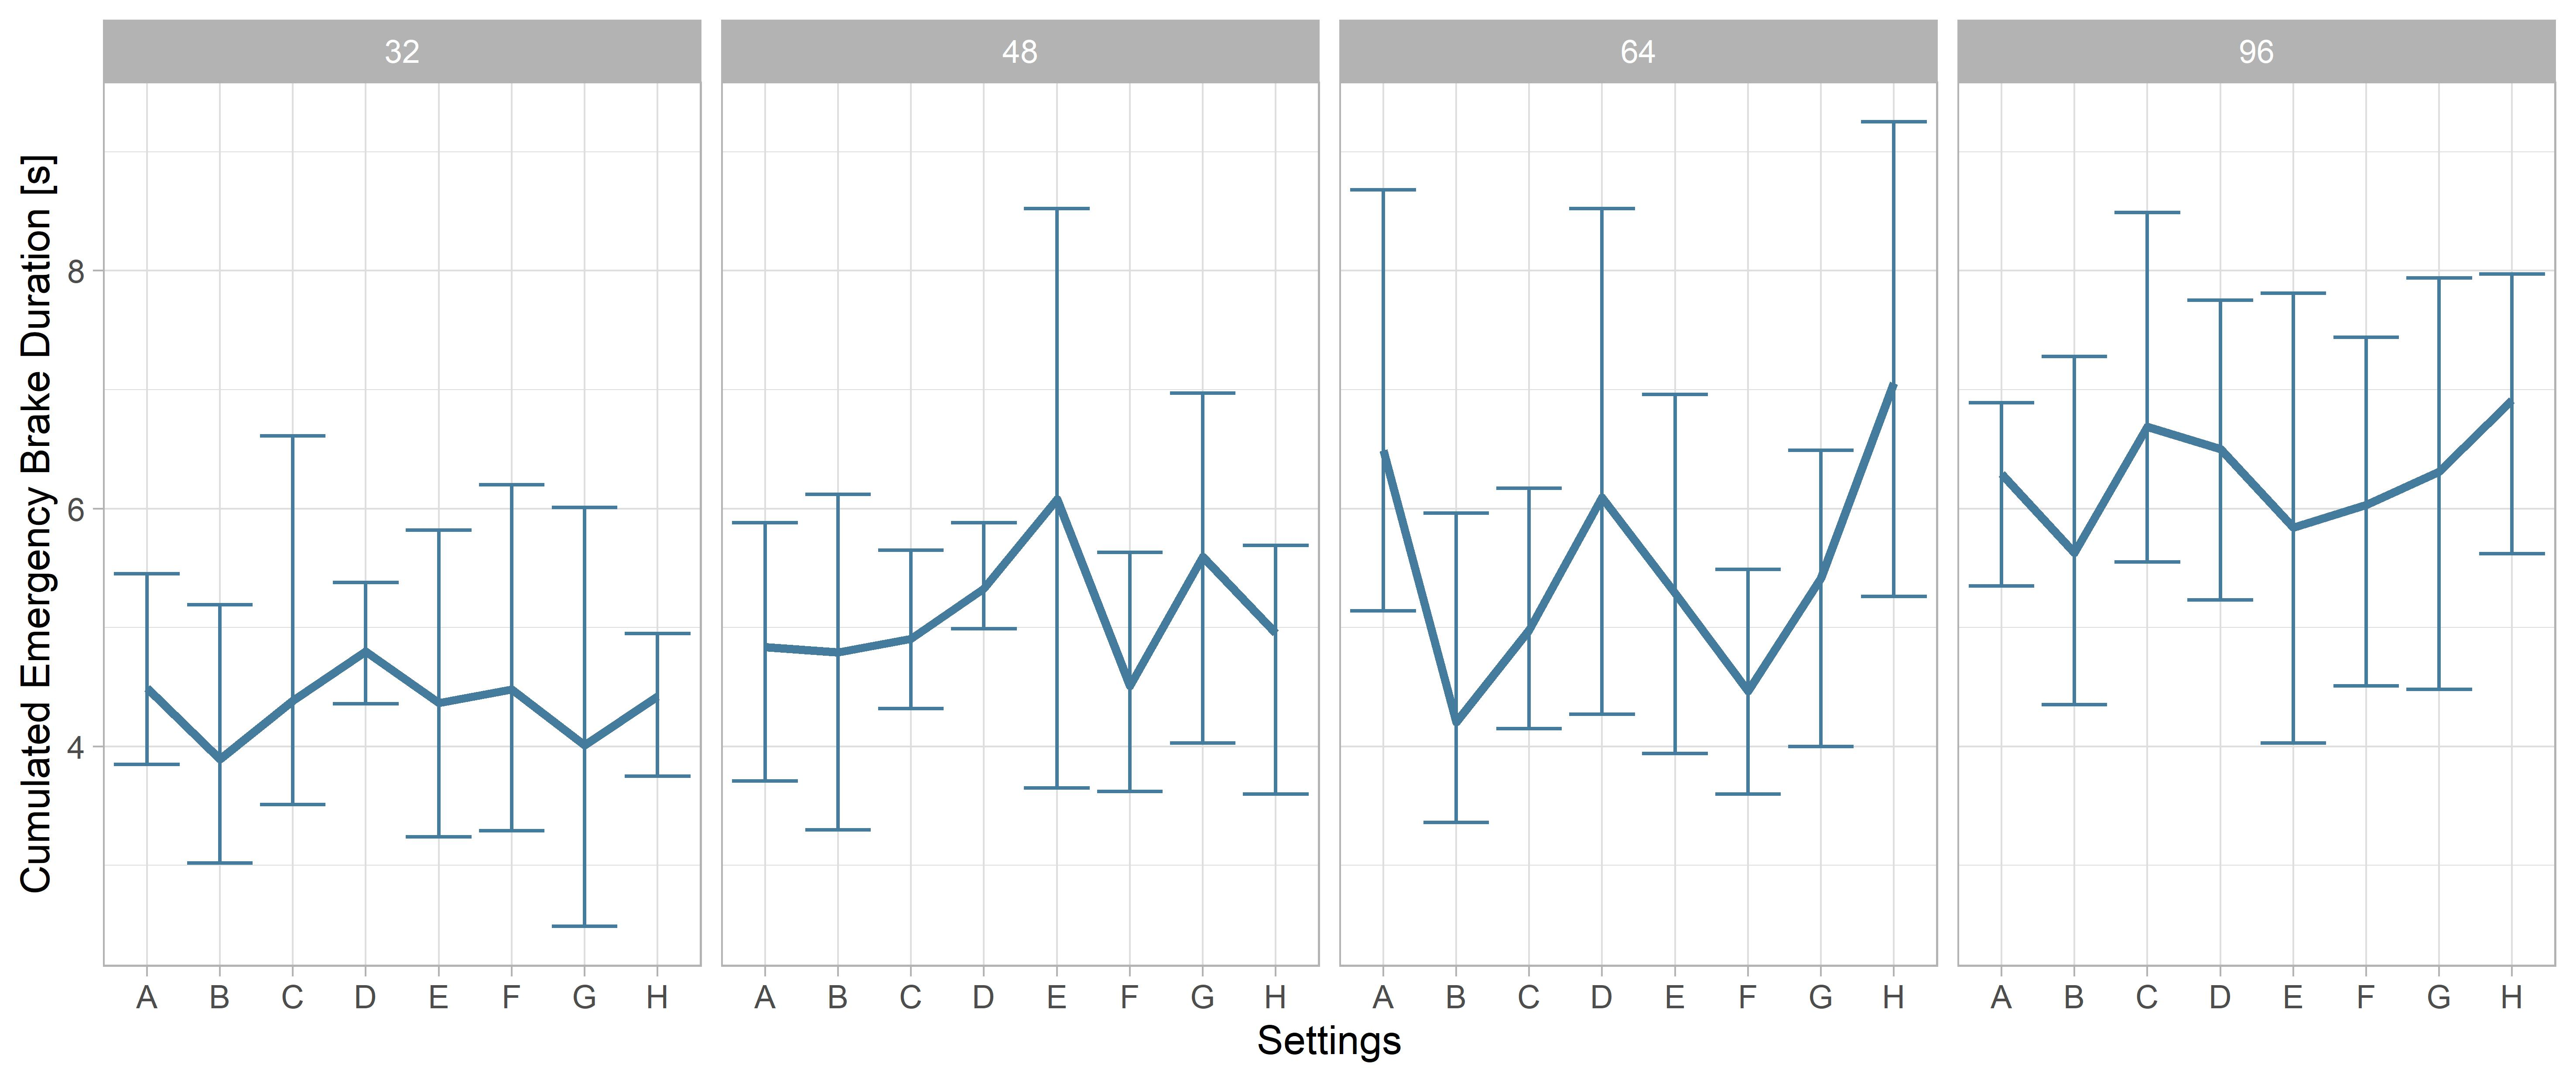
\includegraphics[width=1\linewidth]{simulations/population/plots/comparison}
	\caption{mean and error bars per population}
		\label{figure:population:results}
\end{figure}


A higher spread in the results can be seen when looking at small population sizes. Considering these findings, a population size of 96 was chosen. While such a high value will result in a performance impact, it was deemed to be more important to keep the variation low.


\section{Design of Experiment}
\label{chap:hyperparameter_tuning:other_parameter}

This section mains to find optimal settings for the remaining control parameters for the given problem.
Following the conclusion from the previous section \ref{chap:hyperparameter_tuning:population}, a population size of 96 will be used. 

In order to tune the control parameter of the genetic algorithm, various different strategies can be used. Using automated approaches like "Grid Search", "Bayesian Optimization, "Simmulated Annealing or "Hyperband" might lead to good results with minimal effort (tuning hyperparameter of these search algorithms is still needed), however they each require a high number of runs (\cite{kacprzyk_parameter_2007}).\todo{find more (better) references} \cite{kacprzyk_parameter_2007} even suggest using a second, higher level Genetic Algorithm for the optimization process.

Due to performance considerations, many optimization methods however did not fit the requirements.
Executing one run for 30 generations currently takes around 3:50 hours. Although two different workstations were available, the time required to execute the needed number of runs for these automated tests would exceed the available time budged. This is without considering a minimum required number of repetitions to remove randomness in the results.


A different approach called "design of experiment" (DOE), also known as statistically designed experiments. DOE tries to find the cause and-effect relationship between the factors and the output of experiments.
It uses factorial design where each experiment has factors, of which each consists of at least two settings, with the actual number of settings being called "levels" (\cite{yang_design_2009}). Design of experiment needs manual expertise to define which factors are possibly of importance and which settings each factor should have.

\enquote{If the range of variable is too small, then we may miss lots of useful information. If the range is too large, then the extreme values might give infeasible experimental runs.} (\cite{yang_design_2009})

Afterwards, main effects and interactions can be calculated to find the best settings per factor. It provides a graphical representation of these relationship by using interaction as well as main-effects charts.
Using ANOVA (Analysis of Variance) it is possible to identify the significance of each factor and interaction, which enables the ranking of these factors. More details on these analysis tools will be provided in section \ref{chap:hyperparameter_tuning:analysis_of_results}.

A full factorial design will test over all possible combinations of the manually selected factor levels. Looking at the proposed factors in table \ref{table:hyperparameter_tuning:settings_to_level}, we would require 1024 runs\footnote{number of runs calculated using: \url{https://datatab.net/statistics-calculator/design-of-experiments}}, which not feasible performance wise. A full factorial design has the drawback, that as the number of factors k gets increased, the number of needed experimental runs increases exponentially, thus resulting in lengthy experiments. \cite{yang_design_2009} state, that most of the results obtained by testing over all combinations are only used for estimating higher-order interactions, which are in most cases insignificant.

Fractional factorial experiments require less runs ... \todo{Short explaination}

\enquote{Techniques such as fractional (or partial) factorial experiments are used to simplify the experiment. Fractional factorial experiments investigate only a fraction of all possible combinations. This approach saves considerable time and money but requires rigorous mathematical treatment, both in the design of the experiment and in the analysis of the results. (\cite{roy_primer_1990})}


\subsection{Taguchi Design}
Various improvements to Design of experiment have been but forward by Dr. Genichi Taguchi, such as reducing the influence of uncontrollable (noise) factors on processes and products and reducing variability. Some of these methods evolve around Signal-to-noise (S/N) analysis and utilizing cost functions to "express predicted improvements from DOE results in terms of expected cost saving" (\cite{roy_primer_1990}). This master thesis will not discuss all of Taguchi's proposed considerations, for more detail \cite{roy_primer_1990} as well as \cite{yang_design_2009} is highly recommended.

\todo{Find examples of Papers that use taguchi for ga}

Using a Taguchi design for evaluating the best hyperparamter has been successfully performed by \cite{dao_maximising_2016} as well as \cite{naruka_parameter_2019}. 

\enquote{ There are many similarities between “regular” experimental design and Taguchi's experimental design. However, in a Taguchi experiment, only the main effects and two-factor interactions are considered. Higher-order interactions are assumed to be nonexistent. In addition, experimenters are asked to identify which interactions might be significant before conducting the experiment, through their knowledge of the subject matter.} (\cite{yang_design_2009})

This masters thesis will mainly utilizes Taguchis orthogonal arrays (OAs), "which represent the smallest fractional factorials and are used for most common experiment designs." (\cite{roy_primer_1990}). This means, that only a fraction of combinations needs to be tested which drastically improves performance. Each row of these matrices contains the factors of one experiment, while the columns correspond the factors \cite{li_taguchi_2021}. 

Different orthogonal arrays have been proposed by Taguchi. The researcher has the responsibility to select an array based on the individual needs (\cite{li_taguchi_2021}).
Using these orthogonal arrays instead of full factorial experiments will lead to needing a much smaller amount of simulation runs (in our case only 16 compared to 1024), while the latter "might not provide appreciably more useful information" \cite{roy_primer_1990}.


An orthogonal array has multiple properties:
\todo{Definition orthogonal array}
"
OFF and OLH experiment designs sample a full factorial design space in a balanced and orthogonal fashion. Balance ensures good effect estimates by reducing an estimator’s bias and variability. Orthogonality ensures good estimates of two-term interactions. Balance is achieved by ensuring that each level of every factor occurs an equal number of times in the selected sample. Orthogonality is achieved by ensuring that each pair of levels occurs an equal number of times across all experiment parameters in the selected sample. OFF and OLH designs exhibit good space-spanning properties, which aid screening, sensitivity, and comparative analyses. On the other hand, highly fractionated OFF or OLH designs can have poor space-filling properties, which are necessary for optimization analyses.

"\cite{mills_determining_2015}





As has been stated, probably the biggest drawback of using Taguchi orthogonal arrays is on the one hand to increased manual labour and on the other hand the fact, that higher order interactions ignored.

\cite{roy_primer_1990} explains why this might not be a big problem:
\enquote{Generally speaking, OA experiments work well when there is minimal interaction among factors; that is, the factor influences on the measured quality objectives are independent of each other and are linear. In other words, when the outcome is directly proportional to the linear combination of individual factor main effects, OA design identifies the optimum condition and estimates performance at this condition accurately. If, however, the factors interact with each other and influence the outcome, there is still a good chance that the optimum condition will be identified accurately, but the estimate of performance at the optimum can be significantly off. The degree of inaccuracy in performance estimates will depend on the degree of complexity of interactions among all the factors.}

This is complimented by \cite{yang_design_2009}, who states, that:
\enquote{During many years of applications of factorial design, people have found that higher-order interaction effects (i.e., interaction effects involving three or more factors) are very seldom significant. In most experimental case studies, only some main effects and two-factor interactions are significant.}


However, \cite{kacprzyk_parameter_2007} claim, that "tuning EA parameters can itself be a challenging task since EA parameters interact in highly non-linear ways." It remains to be seen in it is possible to use this method for optimizing parameters of a genetic algorithm.

\paragraph{Selection of orthogonal array}
When choosing a suitable Taguchi orthogonal array, we need to take various factors into account, which can make the process tricky. According to \cite{yang_design_2009}, we will have to follow a three step procedure:

\begin{enumerate}
	\item Calculate the total degree of freedom (DOF). 
	\item Following two rules, standard orthogonal array should be selected:
	\begin{enumerate}
		\item Total DOF need to be smaller than the number of runs provided by the orthogonal array.
		\item All required factor level combinations need to be accommodated by the orthogonal array.
	\end{enumerate}
	
	\item Factors have to be assigned using these rules: 
	\begin{enumerate}
		\item In case the factor level does not fit into the orthogonal array, methods such as column merging and dummy level can be used to modify the original array.
		\item Using the linear graph and interaction table, interactions can be defined. 
		\item In case some columns are not assigned, its possible to keep these columns empty.
	\end{enumerate}
\end{enumerate}


For this genetic algorithm, 7 factors (3 Factors of Level 4 and 4 Factors of Level 2) have been selected. Which factors to choose and with which level was done based on experience gained on section \ref{chap:hyperparameter_tuning:population}. When selecting levels, it is important to have them "as far away from either side of the current working condition as possible."(\cite{roy_primer_1990})
In table \ref{table:hyperparameter_tuning:settings_to_level}, every factor with corresponding levels has been listed,

\begin{figure}[ht]
	\centering
\begin{tabular}{ l|c|cccc }
	\hline
	Factors & Code & Level 1 & Level 2 & Level 3 & Level 4\\
	\hline
	CrossoverType 		& A & one point & two point & uniform 0.1 & uniform 0.5\\
	CrossoverProp    	& B & 0.2 & 0.5 & 0.8 & 0.9\\
	MutationProp   		& C & 0.01 & 0.1 & 0.3 & 0.5\\
	ChromosomeType   	& D & Time & Time+NPC & - & -\\
	GeneType			& E & int & dict & - & -\\
	TournamentSize 		& F & 2 & 4 & - & -\\
	IndMutationProp		& G & 0.1 & 0.5 & - & -\\
	\hline
\end{tabular}
\label{table:hyperparameter_tuning:settings_to_level}
\caption{List of Hyperparamters (Factors) matched to a Code and defined settings (Levels)}
\end{figure}


Using this table, we will now find the best standard orthogonal array in section \ref{chap:hyperparameter_tuning:selection_orthogonal_array}. Before doing so, it is important to state, that Taguchi allows to test for possible (pre determined) two-level interactions (\cite{yang_design_2009}). Analysing interactions comes at a cost of Degrees of freedom. If we look at the table, an interaction between ChromosomeType and GeneType might be of interest. Using the power of hindsight, we know, that a second two factor interaction is possible within our chosen array, thus we will have a look at the interaction between Tournament Size and IndMutationPropability as well.


\subsection{Selection of a suitable standart orthogonal array}
\label{chap:hyperparameter_tuning:selection_orthogonal_array}
The total degree of freedom can be quickly calculated using the rules provided by \cite{yang_design_2009}:

\begin{enumerate}
	\item 1 DOF is always used for the overall mean. 
	\item Each factor has a DOF of NumberOfLevels - 1.
	\item Two-factor interactions use this equation to calculate DOF: $(n_{factor1} - 1)(n_{factor2} - 1)$ where $n$ = number of levels.
\end{enumerate}


This leads to the following calculation for the needed 3 Factors of Level 4 and 4 Factors of Level 2 as well as the two interactions between ChromosomeType-GeneType and TournamentSize-IndMutationProp:

\begin{equation} \label{DOF}
	\begin{split}
		DOF & = 1 + 3 * (3 - 1) + 4 * (2 - 1) + 2 * (2 - 1) * (2 - 1) \\
		& = 13
	\end{split}
\end{equation}

A $L_{16}$ array seems suitable to accommodate the required 13 DOF, which can be seen in \ref{table:hyperparameter_tuning:L16_orhtogonal_array}.


\begin{figure}[ht]
	\centering
\begin{tabular}{ |c||c|c|c|c|c|c|c|c|c|c|c|c|c|c|c|  }
	\hline
	   & \multicolumn{15}{c|}{ $L_{16}(2^{15})$ } \\
	NO.& 1 & 2 & 3 & 4 & 5 & 6 & 7 & 8 & 9 & 10& 11& 12& 13& 14&15\\
	\hline
	1  & 1 & 1 & 1 & 1 & 1 & 1 & 1 & 1 & 1 & 1 & 1 & 1 & 1 & 1 & 1\\
	2  & 1 & 1 & 1 & 1 & 1 & 1 & 1 & 2 & 2 & 2 & 2 & 2 & 2 & 2 & 2\\
	3  & 1 & 1 & 1 & 2 & 2 & 2 & 2 & 1 & 1 & 1 & 1 & 2 & 2 & 2 & 2\\
	4  & 1 & 1 & 1 & 2 & 2 & 2 & 2 & 2 & 2 & 2 & 2 & 1 & 1 & 1 & 1\\
	5  & 1 & 2 & 1 & 1 & 1 & 2 & 2 & 1 & 1 & 2 & 2 & 1 & 1 & 2 & 2\\
	6  & 1 & 2 & 2 & 1 & 1 & 2 & 2 & 2 & 2 & 1 & 1 & 2 & 2 & 1 & 1\\
	7  & 1 & 2 & 2 & 2 & 2 & 1 & 1 & 1 & 1 & 2 & 2 & 2 & 2 & 1 & 1\\
	8  & 1 & 2 & 2 & 2 & 2 & 1 & 1 & 2 & 2 & 1 & 1 & 1 & 1 & 2 & 2\\
	9  & 2 & 1 & 2 & 1 & 2 & 1 & 2 & 1 & 2 & 1 & 2 & 1 & 2 & 1 & 2\\
	10 & 2 & 1 & 2 & 1 & 2 & 1 & 2 & 2 & 1 & 2 & 1 & 2 & 1 & 2 & 1\\
	11 & 2 & 1 & 2 & 2 & 1 & 2 & 1 & 1 & 2 & 1 & 2 & 2 & 1 & 2 & 1\\
	12 & 2 & 1 & 2 & 2 & 1 & 2 & 1 & 2 & 1 & 2 & 1 & 1 & 2 & 1 & 2\\
	13 & 2 & 2 & 1 & 1 & 2 & 2 & 1 & 1 & 2 & 2 & 1 & 1 & 2 & 2 & 1\\
	14 & 2 & 2 & 1 & 1 & 2 & 2 & 1 & 2 & 1 & 1 & 2 & 2 & 1 & 1 & 2\\
	15 & 2 & 2 & 1 & 2 & 1 & 1 & 2 & 1 & 2 & 2 & 1 & 2 & 1 & 1 & 2\\
	16 & 2 & 2 & 1 & 2 & 1 & 1 & 2 & 2 & 1 & 1 & 2 & 1 & 2 & 2 & 1\\
	\hline
\end{tabular}
\label{table:hyperparameter_tuning:L16_orhtogonal_array}
\caption{ $L_{16}(2^{15})$ Taguchi ortohogonal array taken from \cite{roy_primer_1990}}
\end{figure}


This graph now needs to be fitted and modified to accommodate the needed factors. 4 Level Factors need additional space which will be generated using column merging, while interactions will need to be assigned as well.
For this, either an interaction table or linear graphs of the $L_{16}$ array can be used (\cite{nazandanacioglu_taguchi_2005}). 
The linear graph approach is straight forward and will be selected. While there are multiple linear graphs for $L_{16}$ array, \ref{figure:hyperparameter_tuning:linear_graph} describes the graph which best fits the requirements from table \ref{table:hyperparameter_tuning:settings_to_level}. If no graph with the perfect fit is found, theses graphs can be modified as well, using rules described by \cite{nazandanacioglu_taguchi_2005}.

"In each of Taguchi’s orthogonal arrays, there are one or more accompanying linear graphs. A linear graph is used to illustrate the interaction relationships in the orthogonal array."\cite{yang_design_2009}

\begin{figure}[H]
	\label{figure:hyperparameter_tuning:linear_graph}
	\centering
\begin{tikzpicture}
	% Define 1 2 3
	\node (Node2) at (0,0) {2};
	\node (Middle12) at (0,1) {};
	\node (Eclipse12) at (-0.8,0) {};
	\node (Node1) at (0,2) {1};
	
	\draw (Node2) -- node[midway, right] {3} (Node1);
	
	
	% Define 4 8 12
	\node (Node8) at (2,0) {8};
	\node (Middle84) at (2,1) {};
	\node (Eclipse84) at (1.2,0) {};
	\node (Node4) at (2,2) {4};
	
	\draw (Node8) -- node[midway, right] {12} (Node4);
	
	% Define 5 15 10
	\node (Node10) at (4,0) {10};
	\node (Middle105) at (4,1) {};
	\node (Eclipse105) at (3.2,0) {};
	\node (Node5) at (4,2) {5};
	
	\draw (Node10) -- node[midway, right] {15} (Node5);
	
	% Define 7 9 14
	\node (Node9) at (6,0) {9};
	\node (Node7) at (6,2) {7};
	
	\draw (Node9) -- node[midway, right] {14} (Node7);
	
	
	% Define 6 11 13
	\node (Node11) at (8,0) {11};
	\node (Node6) at (8,2) {6};
	
	\draw (Node11) -- node[midway, right] {13} (Node6);
\end{tikzpicture}
\caption{ Linear Graph of $L_{16}(2^{15})$ taken from \cite{yang_design_2009}}
\end{figure}


In a Taguchi linear graph, the nodes as well as the connections both represent columns in the orthogonal array. An interaction between to columns that are represented as nodes "comes out to" to the connecting line column \cite{taguchi_taguchis_2005}. This is useful for both analysing interactions between columns as well as combining (merging) interacting columns in case a higher factor is needed.

\paragraph{Column Merging}
A, B and C are both 4 level factors. The currently selected orthogonal only fits 2 level factors. Using column merging, it is possible to extend columns to accomodate higher order levels. 

As calculated in \ref{DOF}, a four-level column requires three degrees of freedom, thus three two-level columns need to be merged. For column merging, it is required, that the to be merged columns are part of an interaction group (\cite{yang_design_2009}).

So, 3 interaction 2-level columns need to first be selected. One column is discarded, the remain two columns need to be merged using the rules in tabular \ref{table:hyperparameter_tuning:merging_rules}.

\begin{figure}[ht]
	\centering
	\begin{tabular}{ |ccccccc|  }
		\hline
		\multicolumn{3}{|c}{ OLD COLUMN } & & & & NEW COLUMN \\
		\hline
		& 1 & 1 & & -> & & 1\\
		& 1 & 2 & & -> & & 2\\
		& 2 & 1 & & -> & & 3\\
		& 2 & 2 & & -> & & 4\\
		\hline
	\end{tabular}
	\caption{Rules taken from \cite{roy_primer_1990}}
	\label{table:hyperparameter_tuning:merging_rules}
\end{figure}

The four-level factor can then be assigned to this newly generated column. Because three four-level factors are needed for the current experiment, nine two-level columns need to be merged in total.

\paragraph{Assigning Interactions}
Interactions between two-level factors can be assigned using the linear graph as well. Here, select two connected nodes. The column describing their connection will subsequently contain the interaction (\cite{taguchi_taguchis_2005}).

An interaction between ChromosomeType and GeneType seems possible, thus D and E will be assigned to connected nodes in the linear graph. As we still have some unused space in the graph, we will also look at the interaction of TournamentSize and IndMutationProp (F and G). The resulting graph can be seen in \ref{figure:hyperparameter_tuning:linear_graph_assigned}.


\begin{figure}[H]
	\centering
	\label{figure:hyperparameter_tuning:linear_graph_assigned}
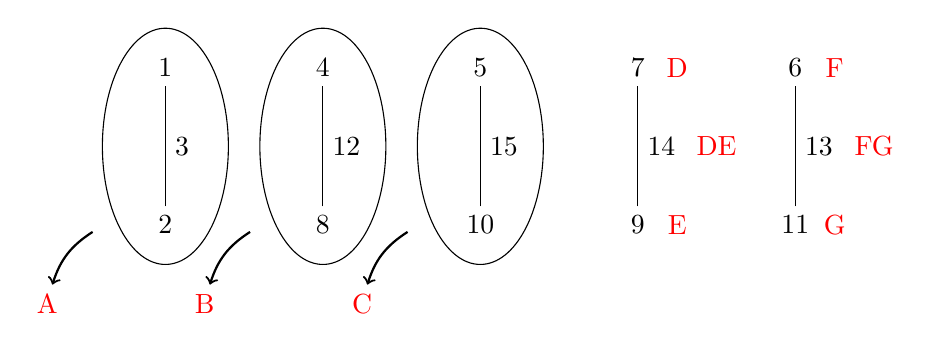
\begin{tikzpicture}
	% Define 1 2 3
	\node (Node2) at (0,0) {2};
	\node (Middle12) at (0,1) {};
	\node (Eclipse12) at (-0.8,0) {};
	\node (Node1) at (0,2) {1};
	\node[red] (A) at (-1.5, -1) {A};

	\draw (Node2) -- node[midway, right] {3} (Node1);
	\draw (Middle12) ellipse (0.8cm and 1.5cm);
	\draw[->, thick] (Eclipse12) to[bend right=20] (A);
	
	
	% Define 4 8 12
	\node (Node8) at (2,0) {8};
	\node (Middle84) at (2,1) {};
	\node (Eclipse84) at (1.2,0) {};
	\node (Node4) at (2,2) {4};
	\node[red] (B) at (0.5, -1) {B};
	
	\draw (Node8) -- node[midway, right] {12} (Node4);
	\draw (Middle84) ellipse (0.8cm and 1.5cm);
	\draw[->, thick] (Eclipse84) to[bend right=20] (B);
	
	% Define 5 15 10
	\node (Node10) at (4,0) {10};
	\node (Middle105) at (4,1) {};
	\node (Eclipse105) at (3.2,0) {};
	\node (Node5) at (4,2) {5};
	\node[red] (C) at (2.5, -1) {C};
	
	\draw (Node10) -- node[midway, right] {15} (Node5);
	\draw (Middle105) ellipse (0.8cm and 1.5cm);
	\draw[->, thick] (Eclipse105) to[bend right=20] (C);
	
	% Define 7 9 14
	\node (Node9) at (6,0) {9};
	\node (Node7) at (6,2) {7};
	\node[red] (E) at (6.5,0) {E};
	\node[red] (D) at (6.5,2) {D};
	\node[red] (DE) at (7,1) {DE};
	
	\draw (Node9) -- node[midway, right] {14} (Node7);
	
	
	% Define 6 11 13
	\node (Node11) at (8,0) {11};
	\node (Node6) at (8,2) {6};
	\node[red] (G) at (8.5,0) {G};
	\node[red] (F) at (8.5,2) {F};
	\node[red] (FG) at (9,1) {FG};
	
	\draw (Node11) -- node[midway, right] {13} (Node6);
\end{tikzpicture}
\caption{Modified Linear Graph to fit our needs}
\end{figure}


Combining columns 1 2 3 to A, 4 8 12 to B and 5 10 15 to C using rules defined by table \ref{table:hyperparameter_tuning:merging_rules} is done in \ref{table:hyperparameter_tuning:merging_columns}.

\begin{figure}[ht]
	\centering
	\begin{tabular}{ |c||cccc|cccc|cccc|  }
		\hline
		NO.& 1 & 2 & & \sout{3} & 4 & 8 & &  \sout{12} & 5 & 10 & &  \sout{15}\\
		\hline
		1  & \multicolumn{4}{c}{\sout{1 1} > 1 } & \multicolumn{4}{|c|}{\sout{1 1} > 1 } & \multicolumn{4}{c|}{\sout{1 1} > 1 }\\
		2  & \multicolumn{4}{c}{\sout{1 1} > 1 } & \multicolumn{4}{|c|}{\sout{1 2} > 2 } & \multicolumn{4}{c|}{\sout{1 2} > 2 }\\
		3  & \multicolumn{4}{c}{\sout{1 1} > 1 } & \multicolumn{4}{|c|}{\sout{2 1} > 3 } & \multicolumn{4}{c|}{\sout{2 1} > 3 }\\
		4  & \multicolumn{4}{c}{\sout{1 1} > 1 } & \multicolumn{4}{|c|}{\sout{2 2} > 4 } & \multicolumn{4}{c|}{\sout{2 2} > 4 }\\
		5  & \multicolumn{4}{c}{\sout{1 2} > 2 } & \multicolumn{4}{|c|}{\sout{1 1} > 1 } & \multicolumn{4}{c|}{\sout{1 2} > 2 }\\
		6  & \multicolumn{4}{c}{\sout{1 2} > 2 } & \multicolumn{4}{|c|}{\sout{1 2} > 2 } & \multicolumn{4}{c|}{\sout{1 1} > 1 }\\
		7  & \multicolumn{4}{c}{\sout{1 2} > 2 } & \multicolumn{4}{|c|}{\sout{2 1} > 3 } & \multicolumn{4}{c|}{\sout{2 2} > 4 }\\
		8  & \multicolumn{4}{c}{\sout{1 2} > 2 } & \multicolumn{4}{|c|}{\sout{2 2} > 4 } & \multicolumn{4}{c|}{\sout{2 1} > 3 }\\
		9  & \multicolumn{4}{c}{\sout{2 1} > 3 } & \multicolumn{4}{|c|}{\sout{1 1} > 1 } & \multicolumn{4}{c|}{\sout{2 1} > 3 }\\
		10 & \multicolumn{4}{c}{\sout{2 1} > 3 } & \multicolumn{4}{|c|}{\sout{1 2} > 2 } & \multicolumn{4}{c|}{\sout{2 2} > 4 }\\
		11 & \multicolumn{4}{c}{\sout{2 1} > 3 } & \multicolumn{4}{|c|}{\sout{2 1} > 3 } & \multicolumn{4}{c|}{\sout{1 1} > 1 }\\
		12 & \multicolumn{4}{c}{\sout{2 2} > 3 } & \multicolumn{4}{|c|}{\sout{2 2} > 4 } & \multicolumn{4}{c|}{\sout{1 2} > 2 }\\
		13 & \multicolumn{4}{c}{\sout{2 2} > 4 } & \multicolumn{4}{|c|}{\sout{1 1} > 1 } & \multicolumn{4}{c|}{\sout{2 2} > 4 }\\
		14 & \multicolumn{4}{c}{\sout{2 2} > 4 } & \multicolumn{4}{|c|}{\sout{1 2} > 2 } & \multicolumn{4}{c|}{\sout{2 1} > 3 }\\
		15 & \multicolumn{4}{c}{\sout{2 2} > 4 } & \multicolumn{4}{|c|}{\sout{2 1} > 3 } & \multicolumn{4}{c|}{\sout{1 2} > 2 }\\
		16 & \multicolumn{4}{c}{\sout{2 2} > 4 } & \multicolumn{4}{|c|}{\sout{2 2} > 4 } & \multicolumn{4}{c|}{\sout{1 1} > 1 }\\
		\hline
	\end{tabular}
	\caption{Building 4 Level columns from 2 Level columns}
	\label{table:hyperparameter_tuning:merging_columns}
\end{figure}

Removing the old and inserting the new columns in the table and transcoding 7 to D, 9 to E, 14 to DE, 6 to F, 11 to G and 13 to FG results in the final table \ref{table:hyperparameter_tuning:final_taguchi}.
This combinations table will subsequently be used as settings for the simulation runs.

\begin{figure}[ht]
	\centering
	\begin{tabular}{ |c||c|c|c|c|c|c|c|c|c|  }
		\hline
		NO.& A & B & C & D & E & F & G & FG& DE\\
		\hline
		1  & 1 & 1 & 1 & 1 & 1 & 1 & 1 & 1 & 1\\
		2  & 1 & 2 & 2 & 1 & 2 & 1 & 2 & 2 & 2\\
		3  & 1 & 3 & 3 & 2 & 1 & 2 & 1 & 2 & 2\\
		4  & 1 & 4 & 4 & 2 & 2 & 2 & 2 & 1 & 1\\
		5  & 2 & 1 & 2 & 2 & 1 & 2 & 2 & 1 & 2\\
		6  & 2 & 2 & 1 & 2 & 2 & 2 & 1 & 2 & 1\\
		7  & 2 & 3 & 4 & 1 & 1 & 1 & 2 & 2 & 1\\
		8  & 2 & 4 & 3 & 1 & 2 & 1 & 1 & 1 & 2\\
		9  & 3 & 1 & 3 & 2 & 2 & 1 & 2 & 2 & 1\\
		10 & 3 & 2 & 4 & 2 & 1 & 1 & 1 & 1 & 2\\
		11 & 3 & 3 & 1 & 1 & 2 & 2 & 2 & 1 & 2\\
		12 & 3 & 4 & 2 & 1 & 1 & 2 & 1 & 2 & 1\\
		13 & 4 & 1 & 4 & 1 & 2 & 2 & 1 & 2 & 2\\
		14 & 4 & 2 & 3 & 1 & 1 & 2 & 2 & 1 & 1\\
		15 & 4 & 3 & 2 & 2 & 2 & 1 & 1 & 1 & 1\\
		16 & 4 & 4 & 1 & 2 & 1 & 1 & 2 & 2 & 2\\
		\hline
	\end{tabular}
	\caption{Final version of used Taguchi orthogonal array}
	\label{table:hyperparameter_tuning:final_taguchi}
\end{figure}


\subsection{Analysing the results}
\label{chap:hyperparameter_tuning:analysis_of_results}
Table \ref{table:hyperparameter_tuning:final_taguchi} can now can be used for running all the needed testcases (the interaction columns can be ignored until the evaluation). Transcoding all factors and levels to get the corresponding setting can be done using in the table from \ref{table:hyperparameter_tuning:settings_to_level}. We will repeat every setting 8 times to reduce randomness and gain information about variance. 
Running the Genetic Algorithm using these 16 different settings each repeated 8 times took 10 days on the two previously described workstations\todo{ref to section}.

The results are found in the appendix at \ref{table:appendix:hyperparameter_tuning:final_taguchi}.

\subsubsection{Main-effects and interaction chart}
Identifying the optimal conditions is done by analyzing the main effects per factor. Using them, it is possible to predict the factors, that lead to the best result \cite{roy_primer_1990}.

\cite{yang_design_2009} explains them well: 
\enquote{The main-effects chart is a plot of average responses at different levels of a factor versus the factor levels}

So, for every factor, sum up the mean of all results per level, then divide by the number of runs per level.

\todo{Example for D}

The resulting main-effect charts can be seen here:
\begin{figure}[ht] 
	\label{figure:taguchi:main_effects}
	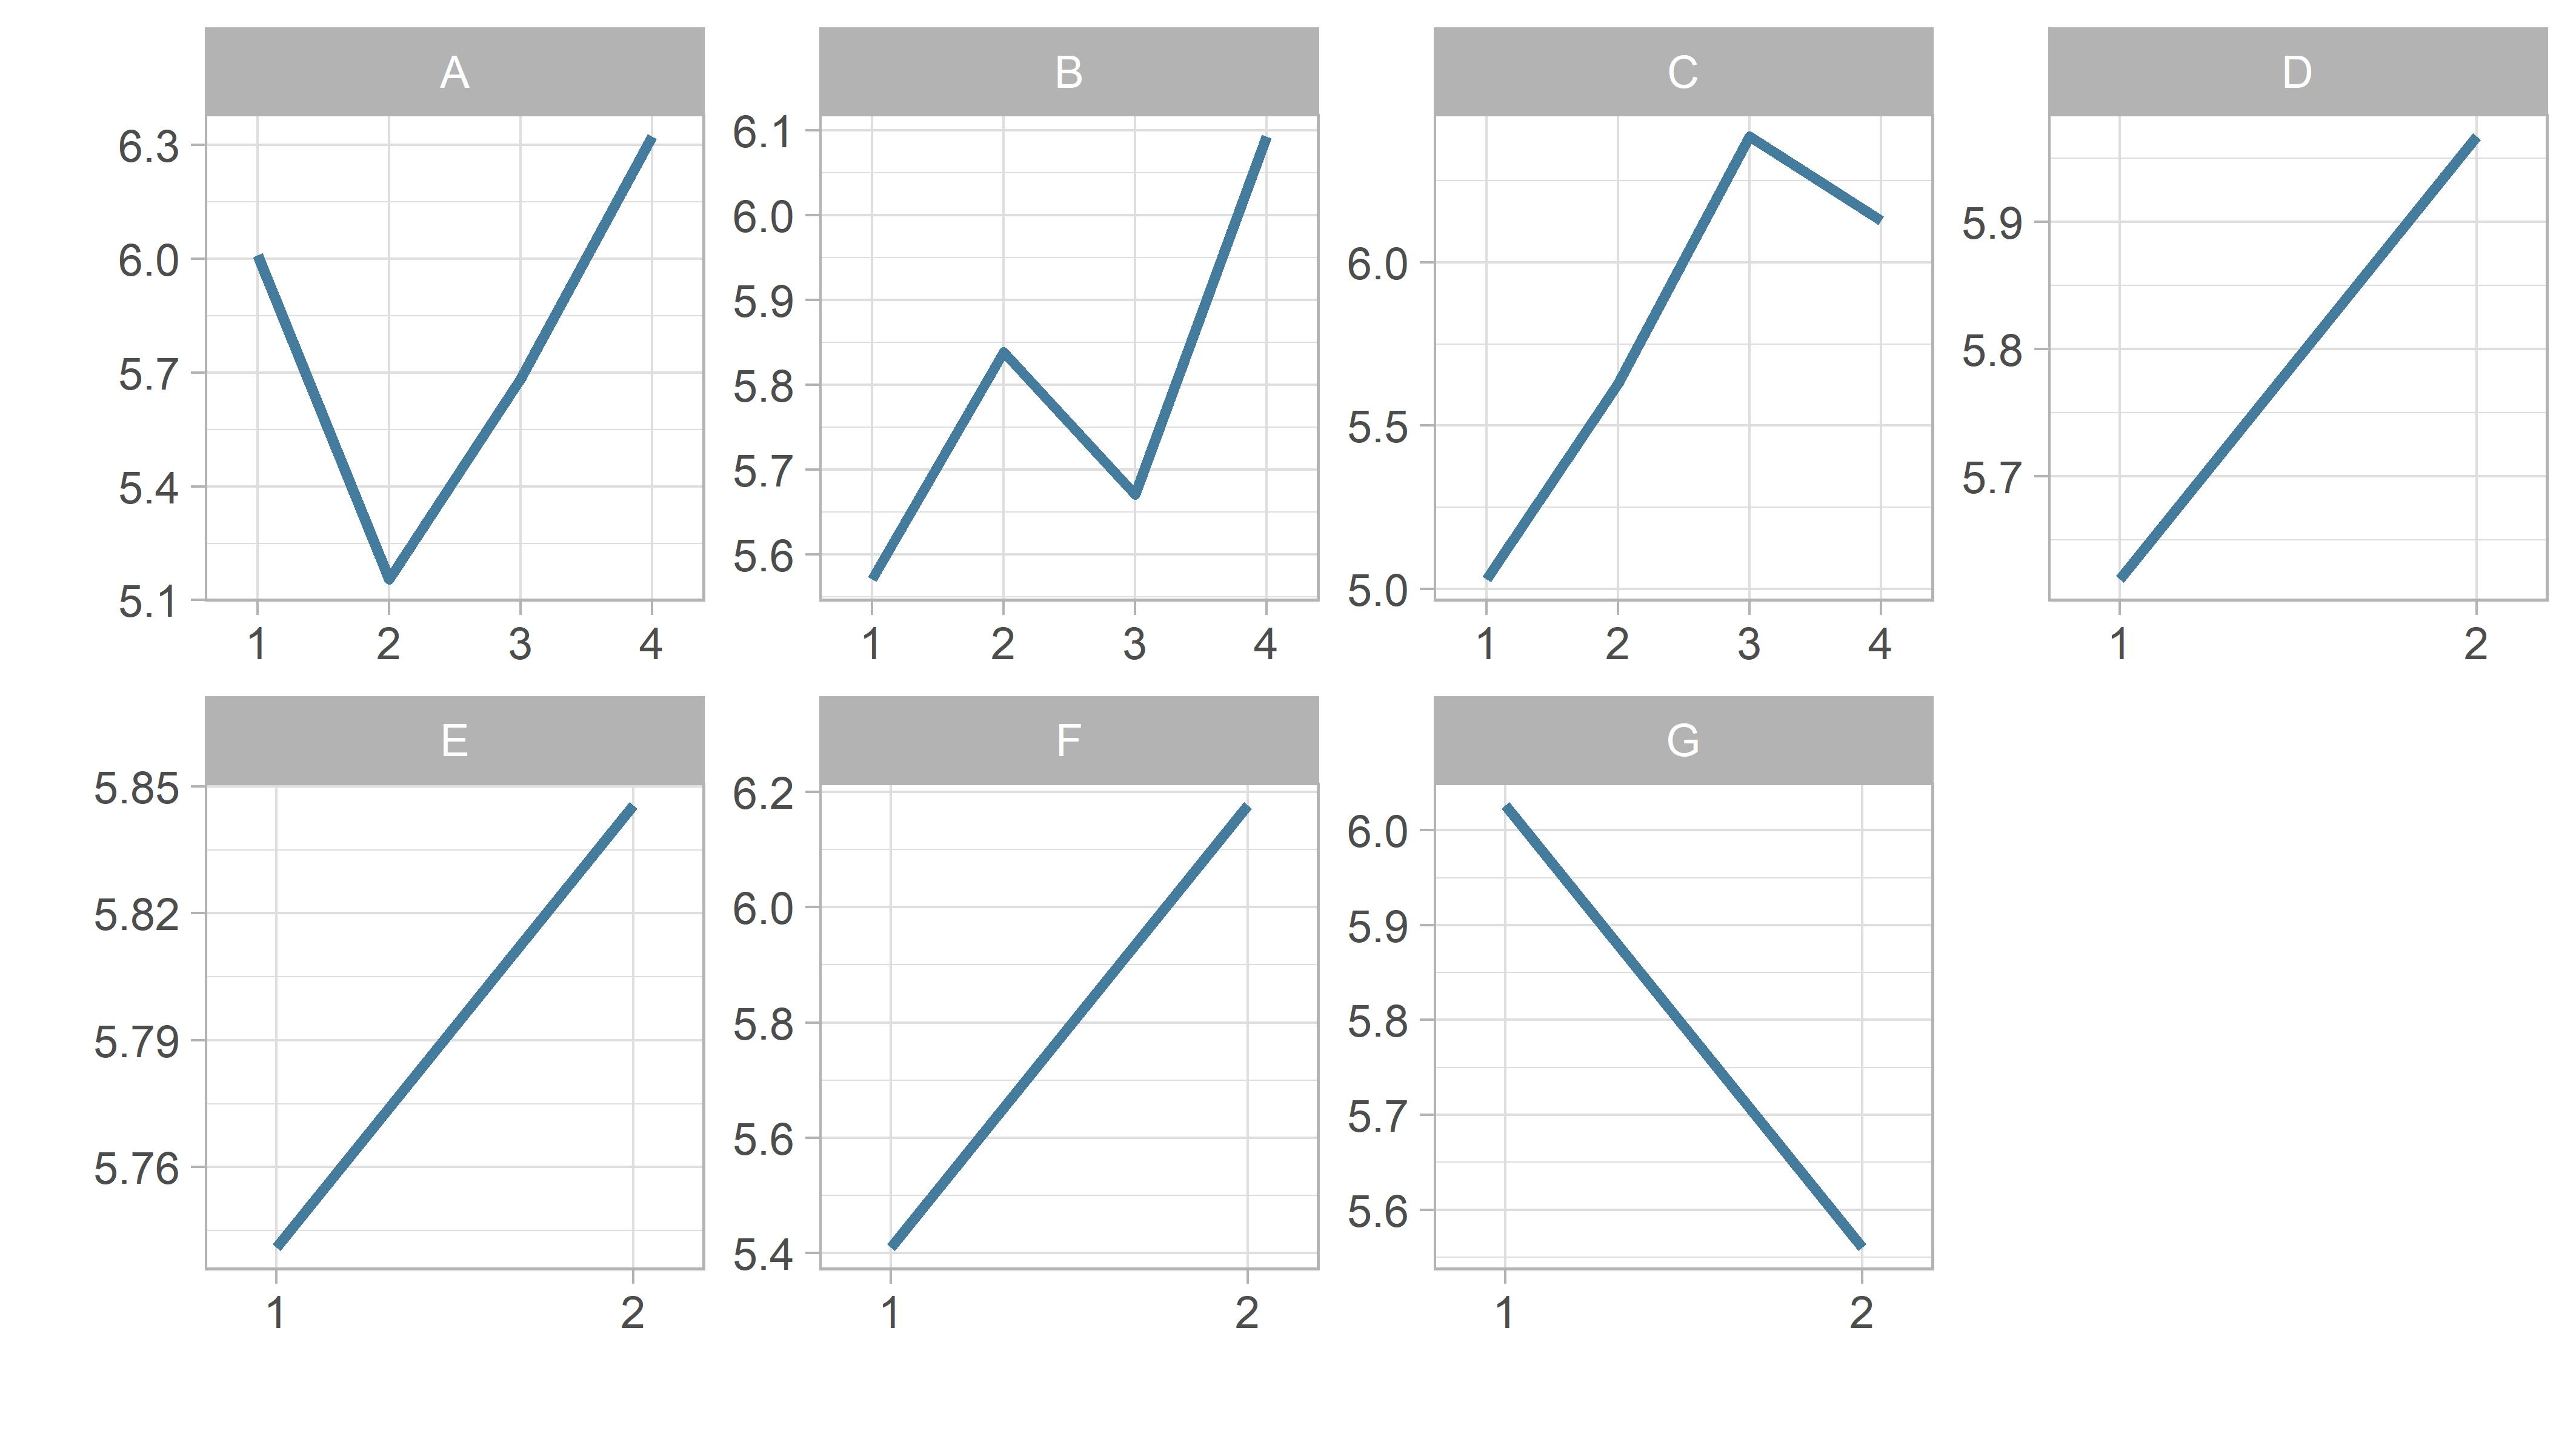
\includegraphics[width=1\linewidth]{simulations/taguchi/plots/main_effects}
	\caption{Main Effects}
\end{figure}


In case there is no interaction, the optimal setting is easily determined by using the main effects chart. Go over every factor in the chart and use the best level (in case of this experiment, the level with the lowest cost value). If interactions exist, they might have an influence on the best settings and need to be investigated (\cite{yang_design_2009}).

To investigate previously defined interactions, a test of interactions can be used. Their calculation is similar to calculating main effects.

\todo{Example for DE}

\begin{figure}[ht] 
	\label{figure:taguchi:test_of_interaction}
	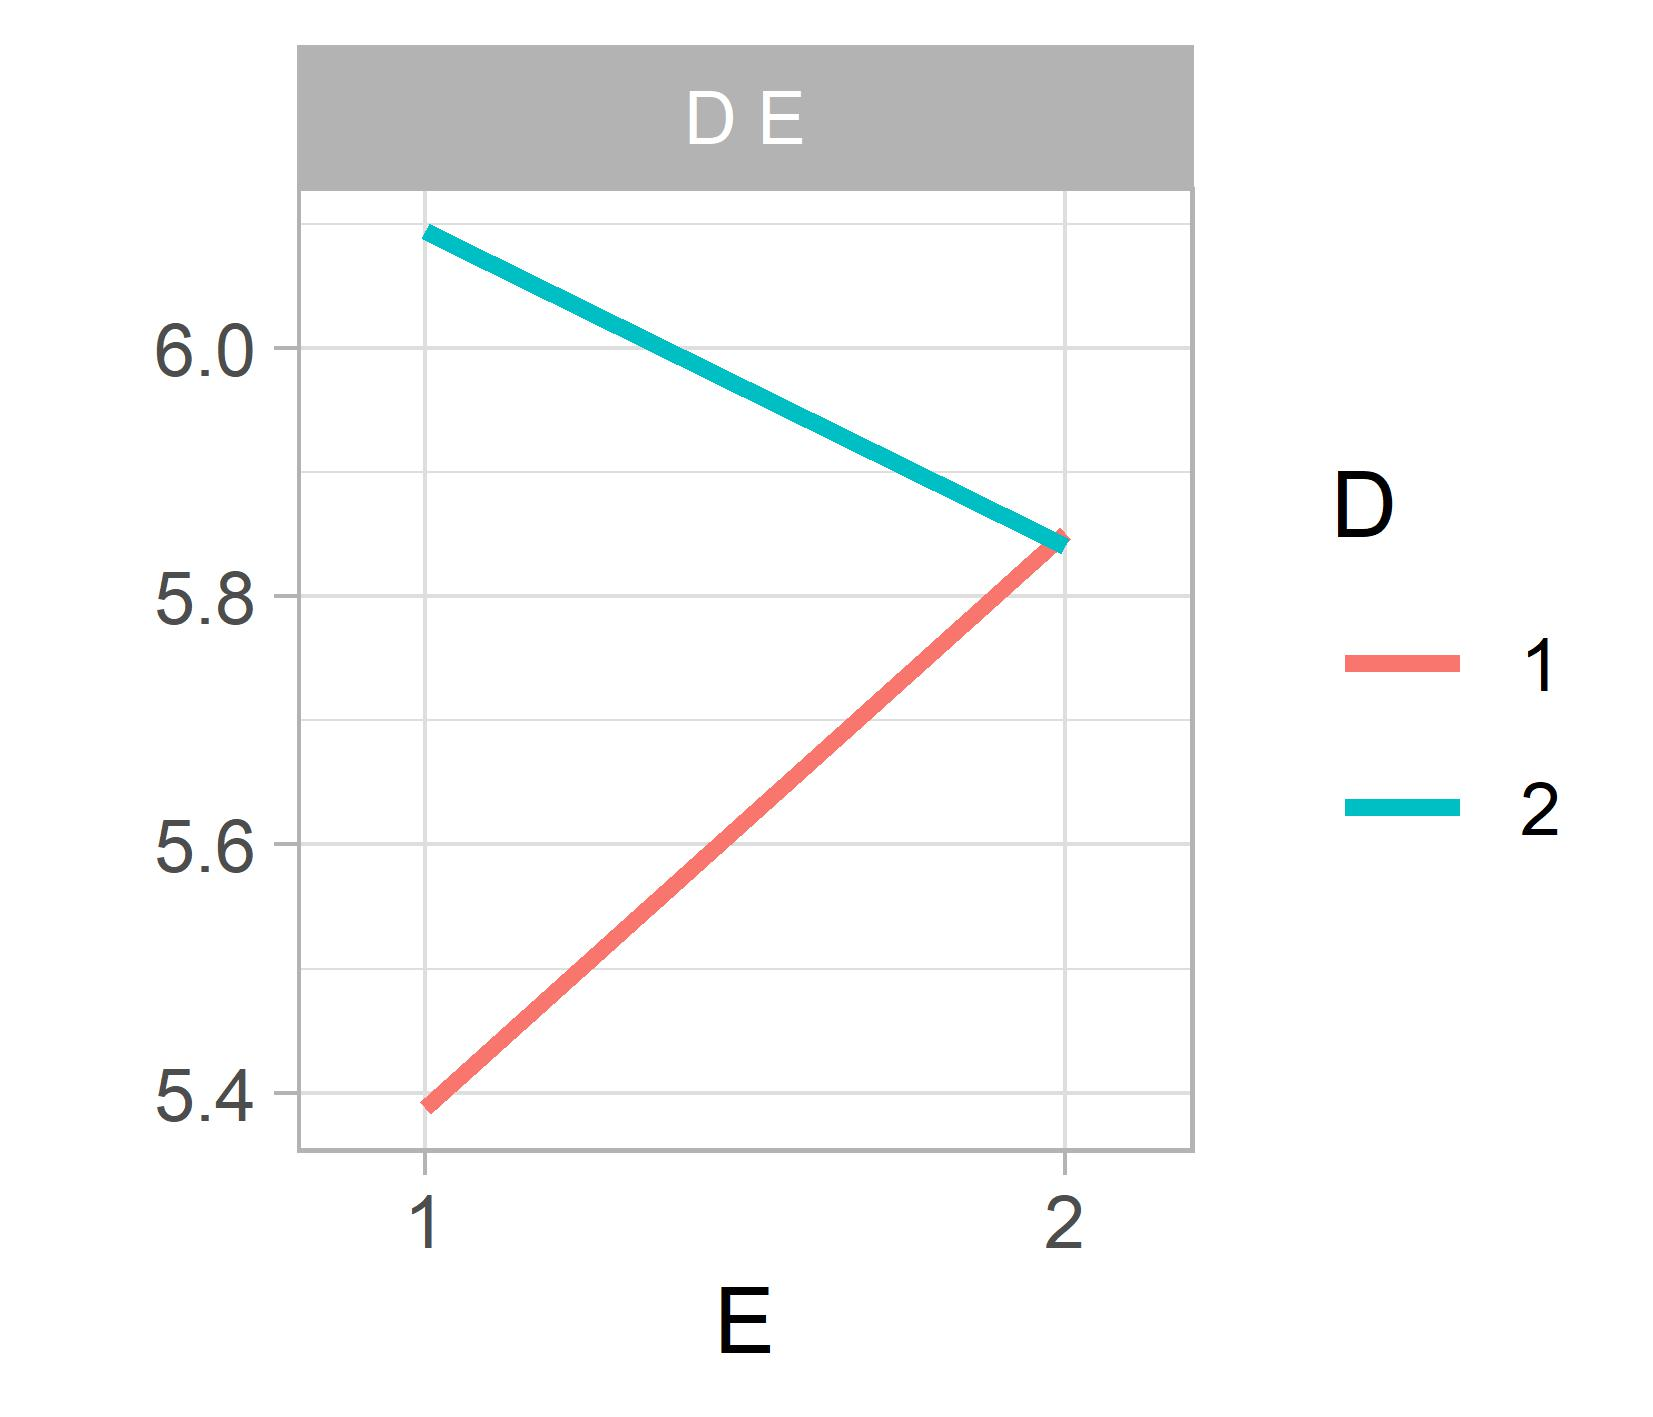
\includegraphics[width=1\linewidth]{simulations/taguchi/plots/test_of_interaction}
	\caption{Test of interactions}
\end{figure}

If lines cross, an interaction between the two factors exists. The more parallel the lines are, the less likely an interaction. Magnitude of the angle between the lines corresponds to the degree of interaction presence, according to \cite{roy_primer_1990}.

\subsubsection{ANOVA}
Before choosing the best settings, ANOVA analysis (analysis of variance) should be performend on the results. Among other things, this will provide information on the magnitude of contribution of each main effects and interactions. The calculation of ANOVA is the same as for a classical design of experiment, according to \cite{yang_design_2009}.

\todo{Summary after reading "Introduction into R"}

"In analysis of variance, mean squares are used in the F test to see if the corresponding effect is statistically significant."\cite{yang_design_2009}
"F ratio is a better measure for relative performance"\cite{yang_design_2009}

". The most commonly used criterion is to compare the p value with 0.05, or 5\%, if p value is less than 0.05, then that effect is significant."\cite{yang_design_2009}

"The variance ratio, commonly called the F statistic, is the ratio of variance due to the effect of a factor and variance due to the error term. (The F statistic is named after Sir Ronald A. Fisher.) This ratio is used to measure the significance of the factor under investigation with respect to the variance of all of the factors included in the error term. The F value obtained in the analysis is compared with a value from standard F-tables for a given statistical level of significance." \cite{roy_primer_1990}.


Due to our number of repetitions, the number of DOF increases according to the following equation (taken from \cite{roy_primer_1990}):
\begin{equation} \label{full DOF}
	\begin{split}
		DOF & = totalNumberOfResults - 1 \\
		& = numberOfTrials * numberOfRepetitions - 1 \\
		& = 16 * 8 - 1 = 127
	\end{split}
\end{equation}


Calculating ANOVA can be done simply be done using R, which will result in table \ref{table:taguchi:anova_results}.

\begin{table}[ht]
	\centering
	\begin{tabular}{lrrrrr}
		\hline
		& Df & Sum Sq & Mean Sq & F value & Pr($>$F) \\ 
		\hline
		A & 3 & 238901.41 & 79633.80 & 6.66 & 0.0004 \\ 
		B & 3 & 49972.09 & 16657.36 & 1.39 & 0.2488 \\ 
		C & 3 & 343169.03 & 114389.68 & 9.56 & 0.0000 \\ 
		D & 1 & 38781.12 & 38781.12 & 3.24 & 0.0745 \\ 
		E & 1 & 3507.03 & 3507.03 & 0.29 & 0.5893 \\ 
		F & 1 & 189112.50 & 189112.50 & 15.81 & 0.0001 \\ 
		G & 1 & 69751.13 & 69751.13 & 5.83 & 0.0174 \\ 
		D:E & 1 & 41041.12 & 41041.12 & 3.43 & 0.0666 \\ 
		F:G & 1 & 26277.78 & 26277.78 & 2.20 & 0.1411 \\ 
		Residuals & 112 & 1339693.00 & 11961.54 &  &  \\ 
		\hline
	\end{tabular}
	\caption{ANOVA results}
	\label{table:taguchi:anova_results}
\end{table}

A, C, F and G have a relatively high F value, which suggests high influence on the model. \todo{explain using R book}

The Multiple R-squared:  0.4275,	Adjusted R-squared:  0.3509 ... both are bad.


We can also look at the percentage contribution of each factor, using the formula gathered by \cite{yang_design_2009}:

\begin{equation} \label{equation:taguchi:ss_t}
	\begin{split}
		SS_T & = SS_A + SS_B + SS_C + ... + SS_{error}
	\end{split}
\end{equation}

\begin{equation} \label{equation:taguchi:contribution}
	\begin{split}
		contribution_A = SS_A / SS_T * 100
	\end{split}
\end{equation}

The percentage contribution is plotted in \ref{figure:taguchi:percentage_contribution} (Sum of all factor contributions == Multiple R-squared in theory)
\begin{figure}[ht] 
	\label{figure:taguchi:percentage_contribution}
	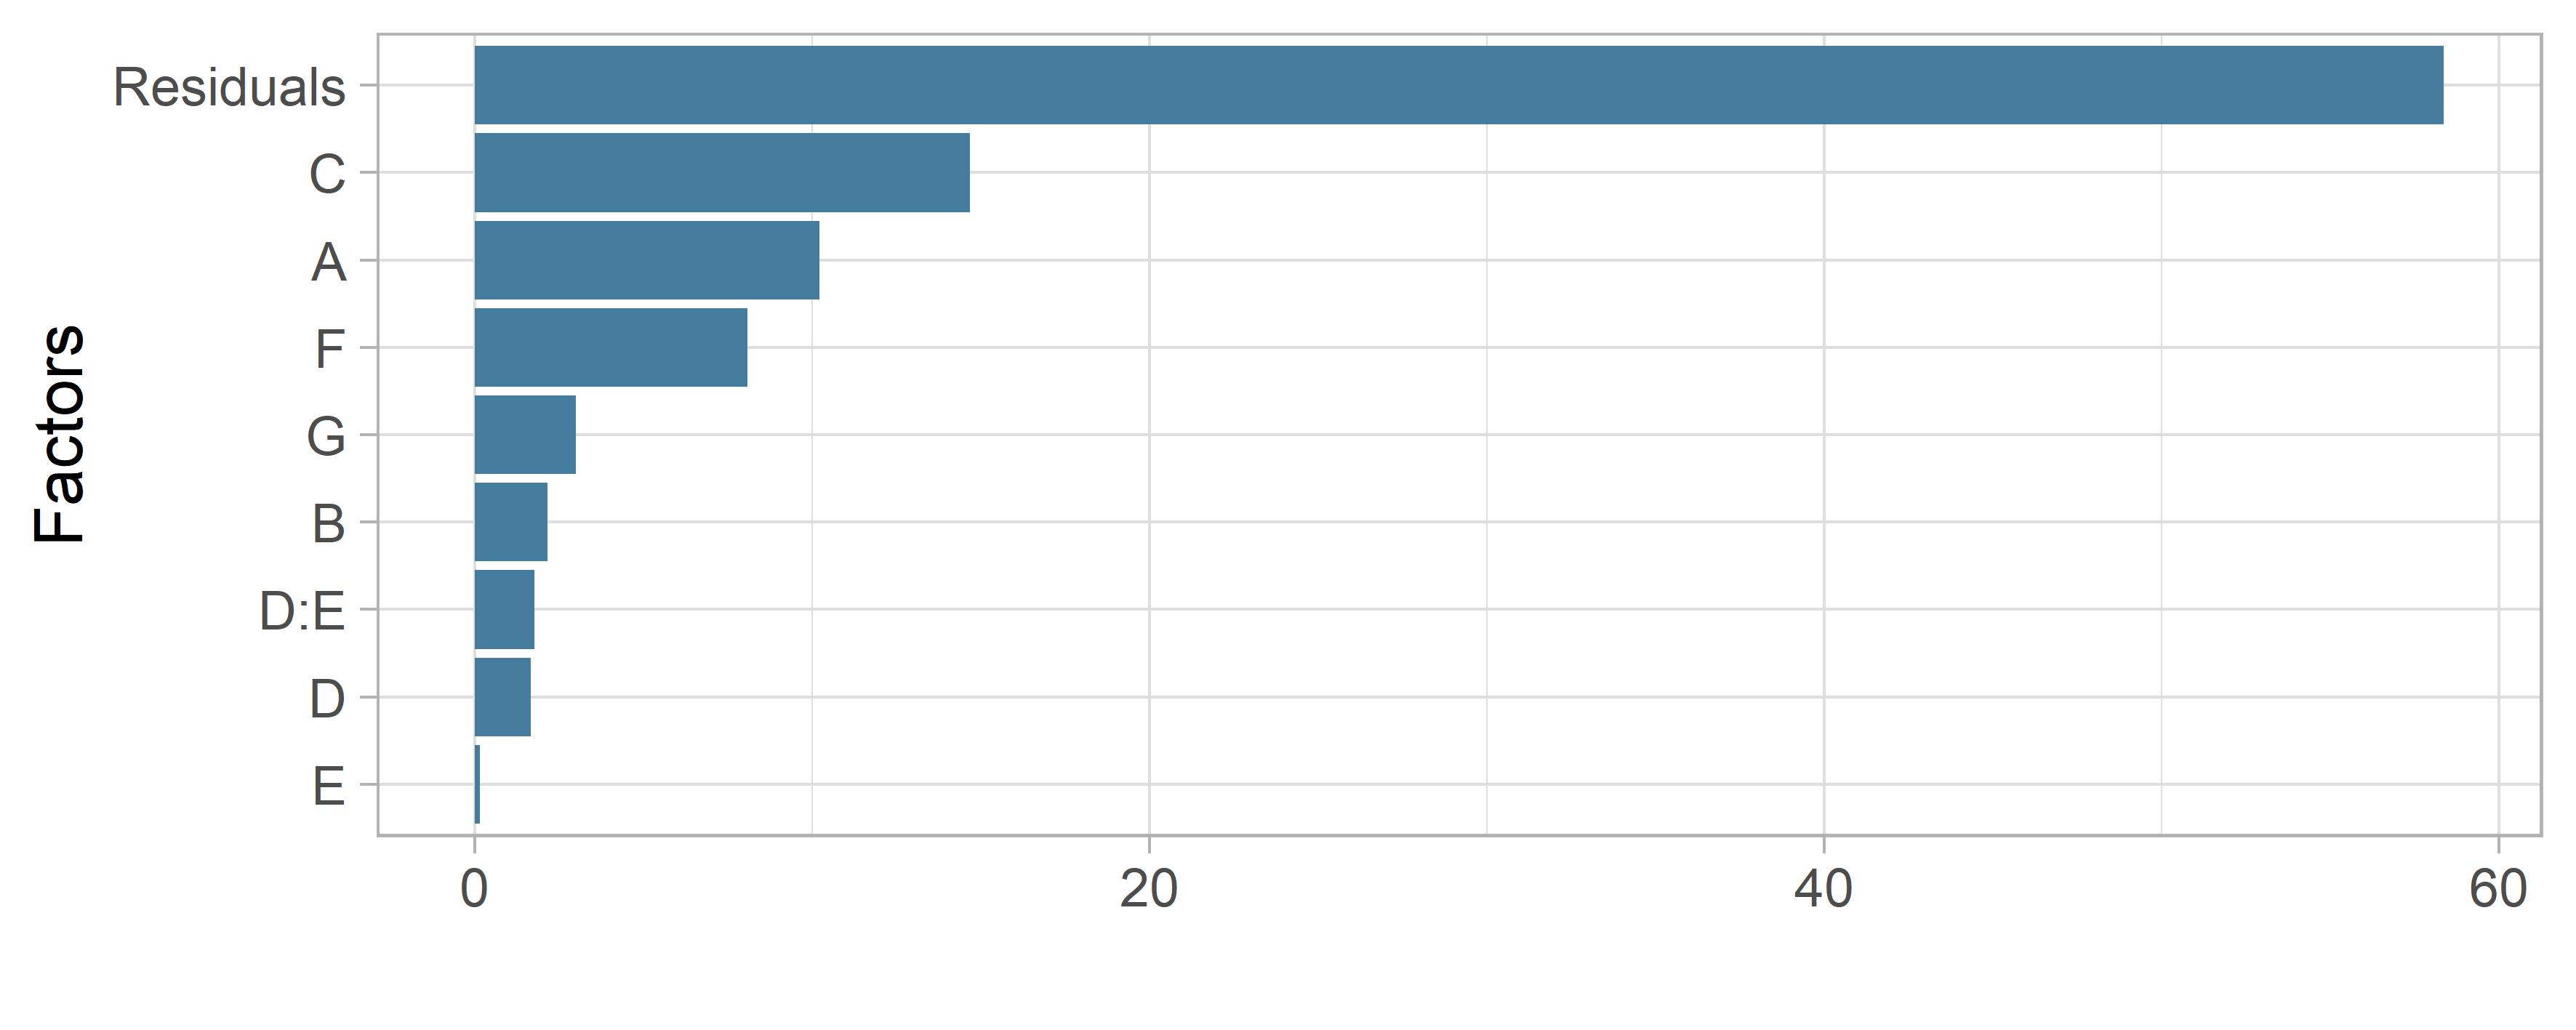
\includegraphics[width=1\linewidth]{simulations/taguchi/plots/percentage_contribution}
	\caption{Percentage Contribution}
\end{figure}

We can clearly see a high contribution of the residuals (error), which is concerning. 

\subsubsection{Selection of optimal setting}
When choosing the optimal setting, the first step is to look at the best main effects combination. For this experiment, the best combination would be the following: A4, B4, C3, D2, E2, F2, G1.
Looking the ANOVA table, the interaction D:E has seams to have significance, especially compared to E. We will try to integrate this interaction. Compared to D:E, the second interaction (F:G) has a lower influence. This is also the case when looking at the individual factors F and G. The interaction F:G will thus not further be discussed.

The test of interaction in figure \ref{figure:taguchi:test_of_interaction} suggest D2 and E1 as the best combination. This is optimal, as D2 is also suggested by the main effects. E1 is different to the suggested main effects, however its low F value in the anova table suggests low significance for using E2.
Concluding this line of thought, the combination A4, B4, C3, D2, E1, F2, G1 looks to be optimal.


\paragraph{Optimum performance calculation}
Using optimal performance calculation 1. using only main effects or 2. using main effects with applied interaction can be applied. The equation provided by \cite{roy_primer_1990}.

\todo{Better bars}
\begin{equation} \label{optimum_perf_main_effect}
	\begin{split}
		Y_{opt} &= \bar{T} + (\bar{A_4} - \bar{T}) + (\bar{B_4} - \bar{T}) + (\bar{C_3} - \bar{T}) + (\bar{D_2} - \bar{T}) + (\bar{E_2} - \bar{T})  + (\bar{F_2} - \bar{T}) + (\bar{G_1} - \bar{T}) \\
			&= 2693.984
	\end{split}
\end{equation}


\begin{equation} \label{optimum_perf_included_interaction}
	\begin{split}
		Y_{opt} &= \bar{T} + (\bar{A_4} - \bar{T}) + (\bar{B_4} - \bar{T}) + (\bar{C_3} - \bar{T}) + (\bar{D_2} - \bar{T}) + (\bar{E_1} - \bar{T})  + ([\bar{DxE}]_2 - \bar{T})  + (\bar{F_2} - \bar{T}) + (\bar{G_1} - \bar{T}) \\
		&= 2686.547
	\end{split}
\end{equation}

Using the interaction D:E, the performance estimation improves from 2693.984 to 2686.547. Considering this result, interaction will be taken into account and the optimized settings are as follows:
CrossoverType: Uniform 0.5, CrossoverPropability: 0.9, MutationPropability: 0.3, ChromosomeType: Time+NPC, GeneType: integer encoding, TournamentSize: 4 and IndividualMutationPropability: 0.1.


\paragraph{signal-to-noise (S/N)}
As previously discussed when looking at the anova model, the error is very high, which suggests high randomness. Taguchi recommends using signal-to-noise (S/N) ratio to reduce the variability, as using only the mean of the results does not take the variation into account (\cite{roy_primer_1990}). The greater the signal-to-noise ratio, the smaller the variance. \cite{roy_primer_1990} further states, that the "use of the S/N ratio offers an objective way to look at the two characteristics (consistency and average value) together."

When using S/N, todo: talk about equation.

Afterwards, generating main effects and anova table is the same as using the mean.
However the DOF calcualtion done in equation \ref{full DOF} is no longer valid, as repetitions get combined to 1 value per run. So, the DOF for anova changes to the following equation in \ref{s_n anova DOF} according to \cite{roy_primer_1990}.

\begin{equation} \label{s_n anova DOF}
	\begin{split}
		DOF & = totalNumberOfResults - 1 \\
		& = numberOfTrials * 1 - 1 \\
		& = 16 - 1 = 15
	\end{split}
\end{equation}

\todo{Find out why 15 DOF is not enough}

This is not enough residuals for generating the F value in anova. Thus in order to reduce the current DOF, the anova table was generated without the interaction F:G considered, which can be seen in \ref{table:taguchi:s_n_anova_results}.

\begin{table}[ht]
	\centering
	\begin{tabular}{lrrrrr}
		\hline
		& Df & Sum Sq & Mean Sq & F value & Pr($>$F) \\ 
		\hline
		A & 3 & 0.26 & 0.09 & 3.01 & 0.3953 \\ 
		B & 3 & 0.05 & 0.02 & 0.60 & 0.7139 \\ 
		C & 3 & 0.38 & 0.13 & 4.44 & 0.3326 \\ 
		D & 1 & 0.04 & 0.04 & 1.48 & 0.4378 \\ 
		E & 1 & 0.00 & 0.00 & 0.12 & 0.7845 \\ 
		F & 1 & 0.21 & 0.21 & 7.35 & 0.2250 \\ 
		G & 1 & 0.08 & 0.08 & 2.80 & 0.3429 \\ 
		D:E & 1 & 0.04 & 0.04 & 1.56 & 0.4296 \\ 
		Residuals & 1 & 0.03 & 0.03 &  &  \\ 
		\hline
	\end{tabular}
		\caption{S/N ANOVA results}
	\label{table:taguchi:s_n_anova_results}
\end{table}


When looking at the p values of this table, it is very obvious that no factor can discard the null - hypothesis, which states that a factor has no significant effect. Considering this, it was deemed to be not necessary to perform further investigations. 
Somehow argument, that having less variablity is only to an extend important. It is always possible to restart a simulation, if the variability is not too large, it is important that the results have a good mean overall. Less variability is in producing products much more important.

\paragraph{Elite}
Although the optimal hyperparameter setting will be discussed in chapter \ref{chap:evaluation}, a problem was obvious when analyzing a run using the optimzed GA. Figure \ref{figure:no_elite} shows for a few selected repetitions the best individual cost per generation.

\begin{figure}[ht] 
	\label{figure:no_elite}
	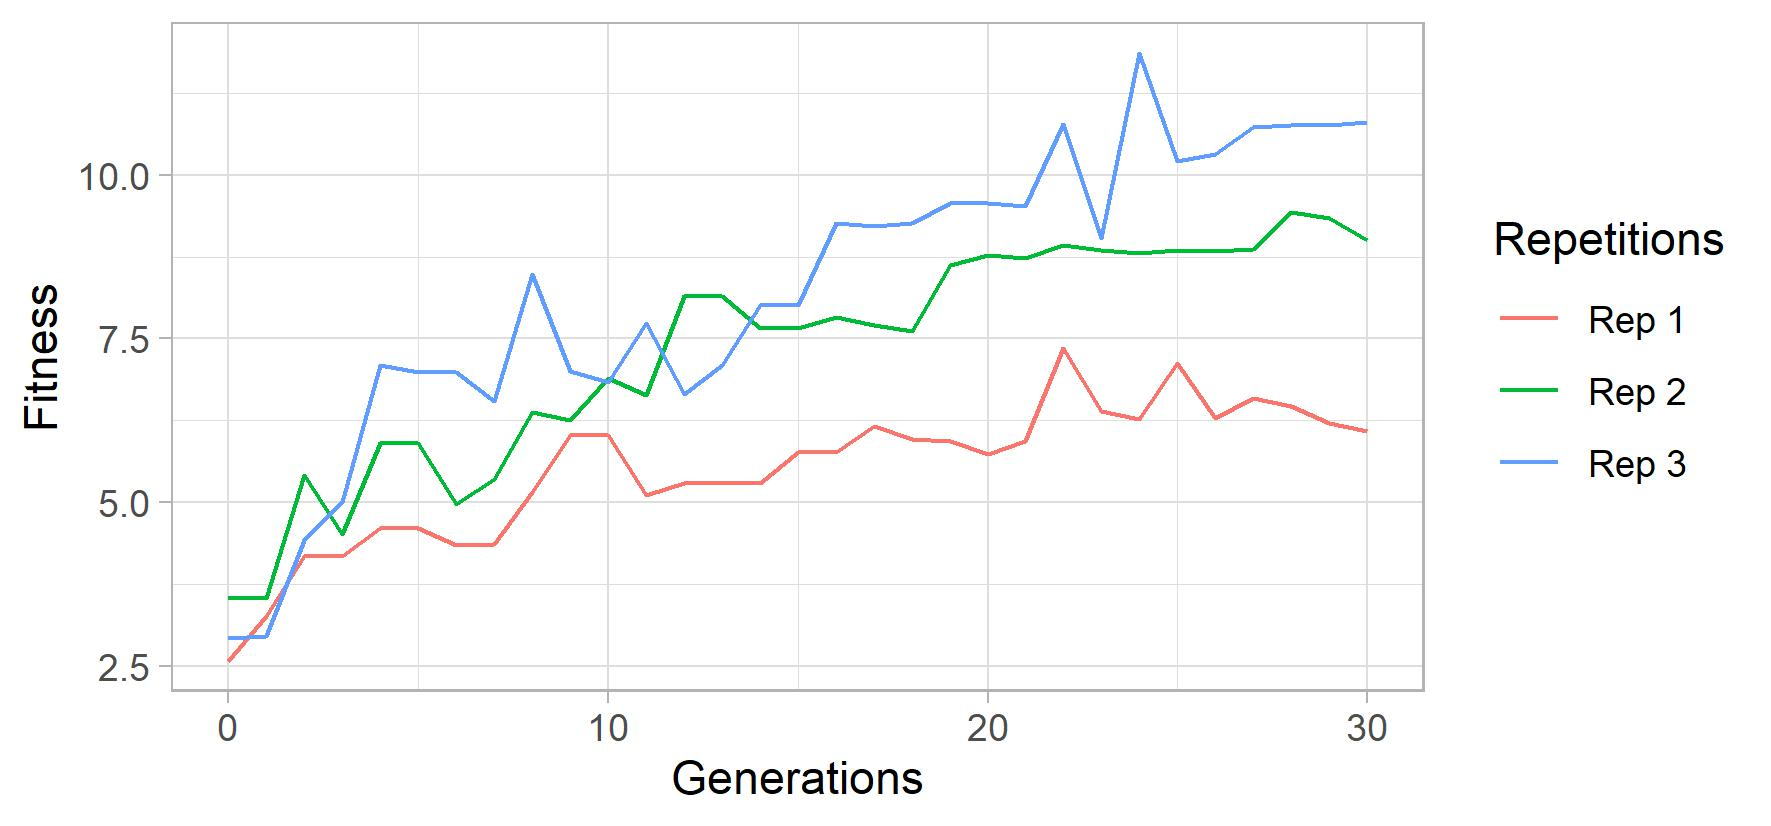
\includegraphics[width=1\linewidth]{simulations/evaluation/plots/ga_no_elite_generations}
	\caption{Genetic Algorithm without Elite}
\end{figure}

The lines show that setbacks in the optimal cost between two generations happens frequenctly. In order to mitigate this problem, it was decided to implement elite selection with a size of 2. This means, that per generation, the two best individuals are copied into the next generation without modifications, which makes worse performance between generations not possible. It is important to note, that the two best individuals can still be selected by tournament selection for modification, its just that a copy of them is saved. Figure \ref{figure:with_elite} shows the effect of these changes.

\begin{figure}[ht] 
	\label{figure:with_elite}
	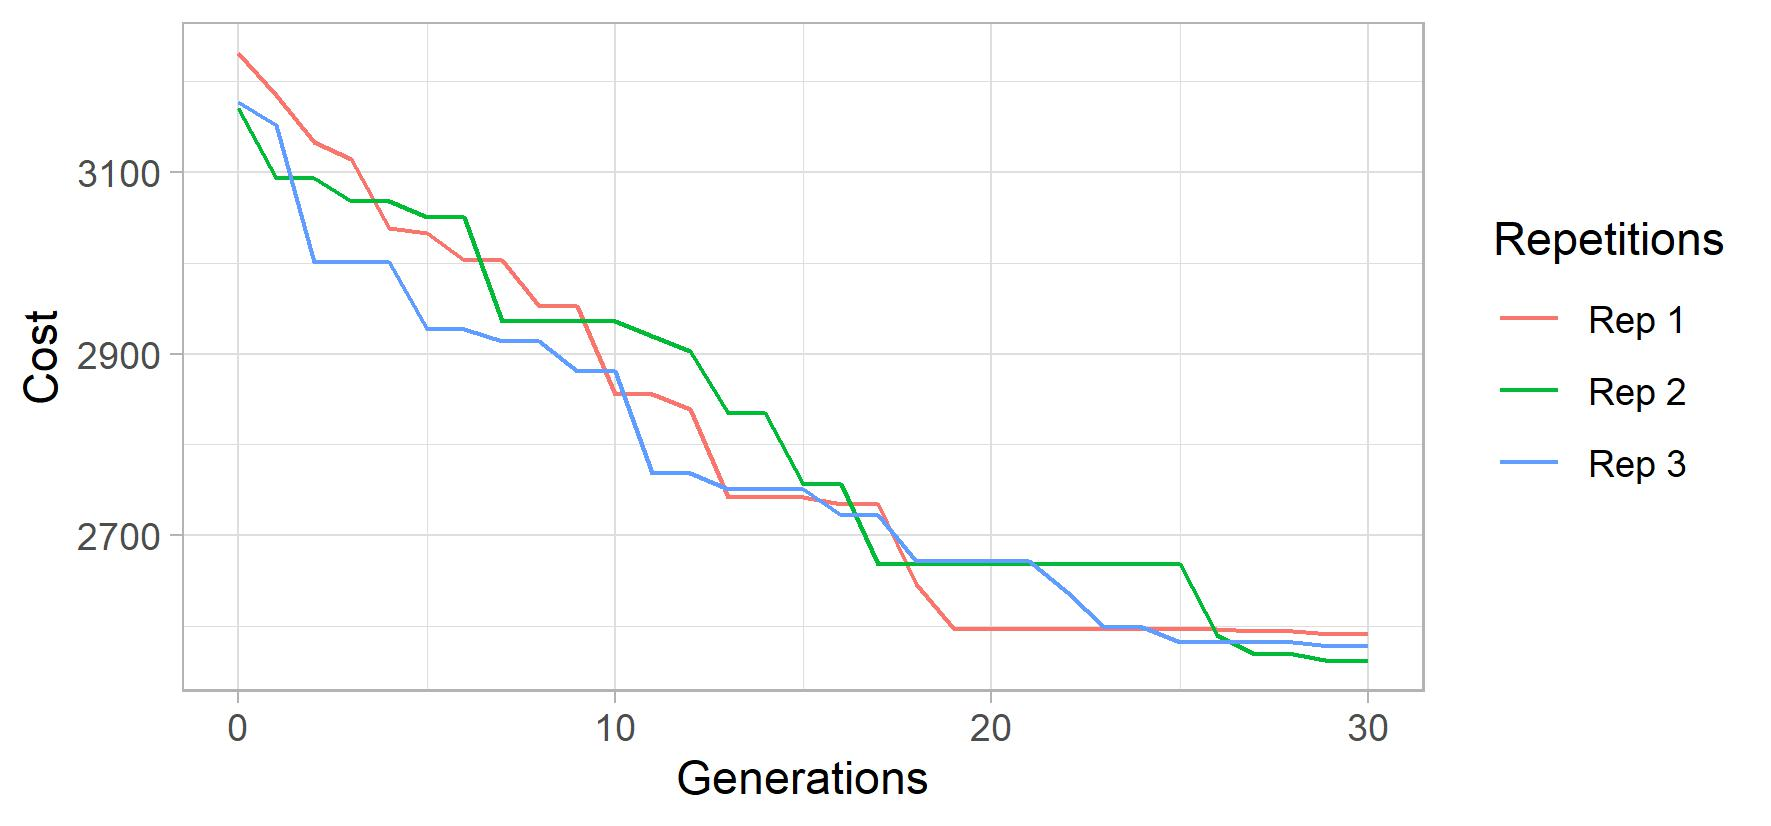
\includegraphics[width=1\linewidth]{simulations/evaluation/plots/ga_elite_generations}
	\caption{Genetic Algorithm with Elite}
\end{figure}


Comparing the 10 repetitions also provides a clear picture in figure \ref{figure:elite_comparison}. It is thus concluded that the slightly modified version of the optimized Ga now using Elite of 2 will be used for chapter \ref{chap:evaluation}.

\begin{figure}[ht] 
	\label{figure:elite_comparison}
	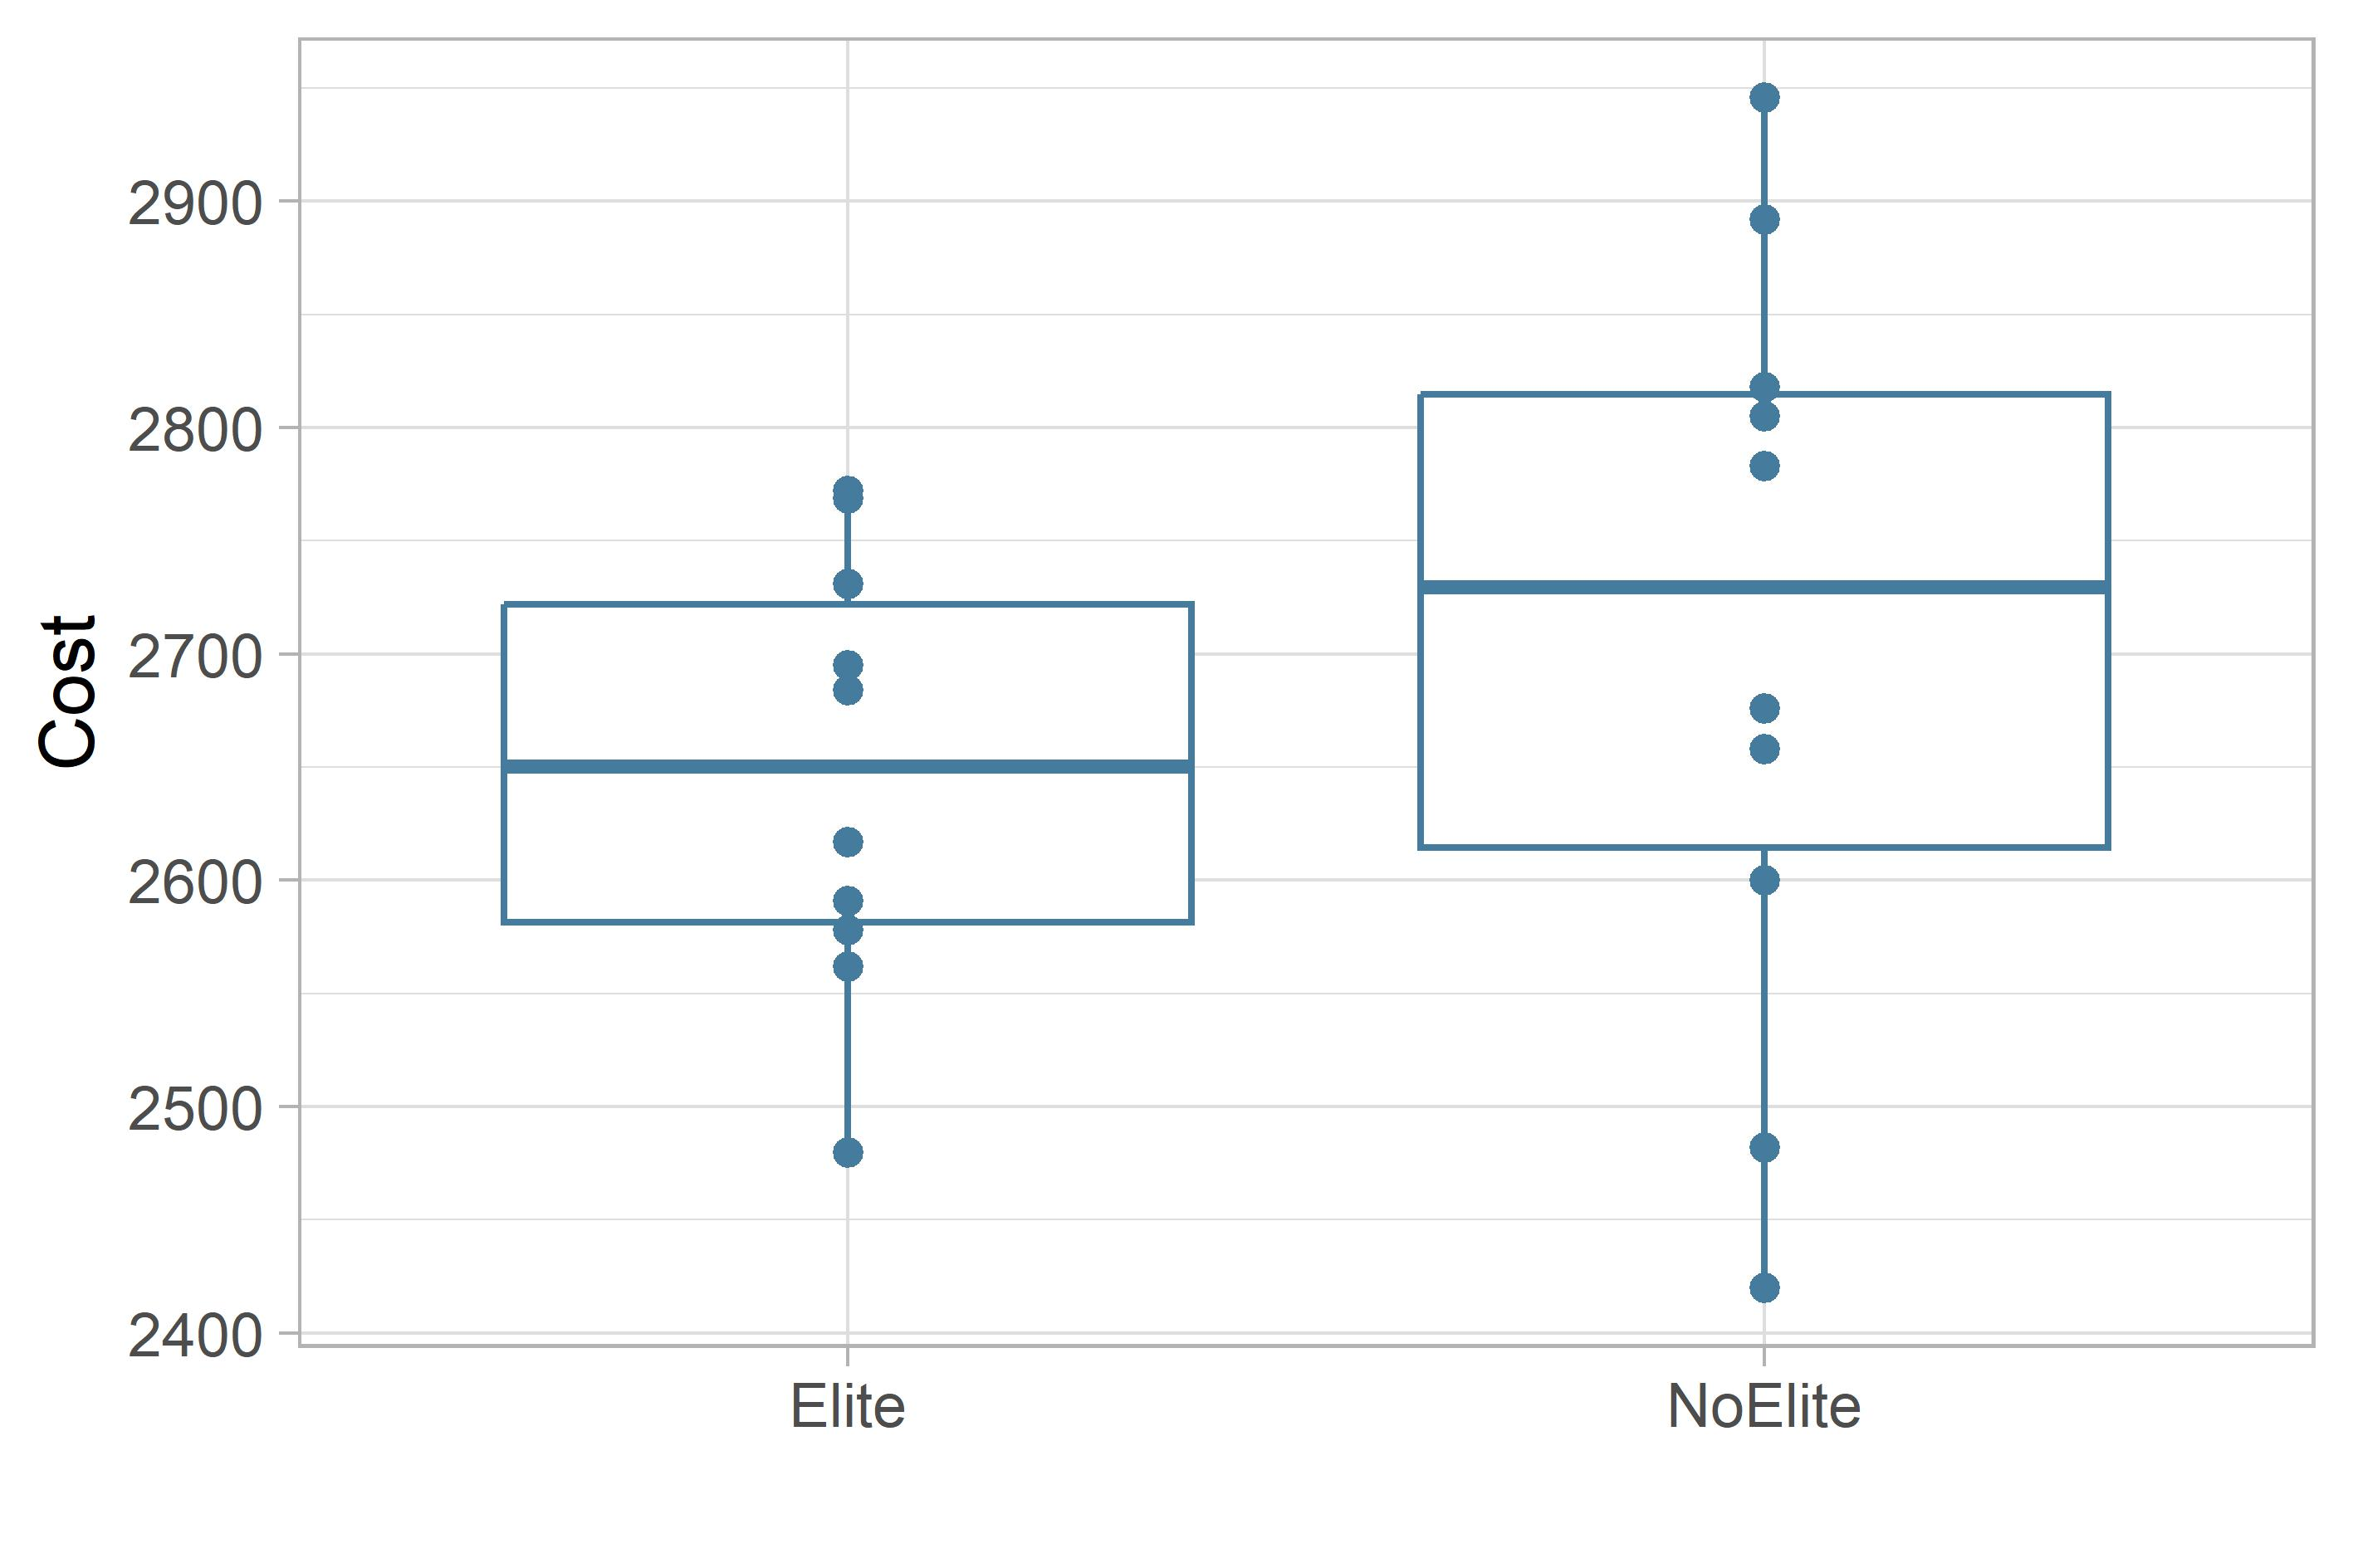
\includegraphics[width=1\linewidth]{simulations/evaluation/plots/elite_vs_no_elite}
	\caption{Comparison Elite vs No Elite}
\end{figure}



